\documentclass[15pt]{beamer}
\usepackage{tikz}
\usepackage{graphicx}
\usepackage{booktabs}
\usetikzlibrary{positioning, arrows.meta}

\usetheme{Berkeley}
\usecolortheme{default}

\title[\LaTeX and Markdown]
{\LaTeX and Markdown}
\author[Matthew, Robson]
{M. ~Robson\inst{1}}

\institute[ICR]
{
  \inst{1}%
  Austin Branch\\
  Institute of Computing in Research
}

\date[July 2026]
{July 2026}


\logo{\begin{tikzpicture}
        \hspace{-0.78cm}
        \raisebox{-0.73cm}{
\includegraphics[width=0.12\textwidth]{logo.jpeg}}
\end{tikzpicture}}

%% finally
\begin{document}

\frame{\titlepage}

\begin{frame}[fragile]
\frametitle{What is a Markup Language?}

\begin{columns}
    \column{0.4\textwidth} 

    \begin{itemize}
        \item HTML
        \item Markdown
        \item \LaTeX
        \item XML
    \end{itemize}
    
    \column{0.6\textwidth}

\begin{block}{\LaTeX}

\begin{verbatim}
\begin{itemize}
    \item First item
    \item Second item
    \item Third item
\end{itemize}
\end{verbatim}
\end{block}

\end{columns}
\vspace{1cm}
Used to help format text in a universal structure.  

\noindent Easy to share as everything is nearly plain text.

\end{frame}
%%%%%%%%%%%%%%%%%%%%%%%%%%%%%%%%%%%%%%%%%%%%%%%%%%%%%%%%%%%%%%%%%%

\begin{frame}[fragile]{Markdown}
Markdown was invented to be a simple format that is easily parseable by any application. It is used in software such as:

\vspace{0.5cm}

\begin{columns}
\column{0.4\textwidth}
    \begin{itemize}
        \item Google Docs
        \item Obsidian
        \item GitHub
        \item Stack Exchange
    \end{itemize}

\column{0.55\textwidth}
\begin{block}{Markdown}

\begin{verbatim}
## Quick start
1. Some list first column
2. something `important`
```python
some code
```
\end{verbatim}
\end{block}


\end{columns}
  
\end{frame}

%%%%%%%%%%%%%%%%%%%%%%%%%%%%%%%%%%%%%%%%%%%%%%%%%%%%%%%%%%%%%%%%%%

\begin{frame}
\frametitle{Pros and Cons}

\begin{columns}

\column{0.5\textwidth}

Pros:
\begin{itemize}
    \item Easy to read documents
    \item Well organized data
    \item Somewhat readable even without using a viewer
    \item Open Source
\end{itemize}

\column{0.5\textwidth}

Cons:
\begin{itemize}
    \item More software requirements
    \item Each standard has different limitations
    \item Can be complex to learn for the first time
\end{itemize}
    
\end{columns}

\end{frame}

%%%%%%%%%%%%%%%%%%%%%%%%%%%%%%%%%%%%%%%%%%%%%%%%%%%%%%%%%%%%%%%%%%

\begin{frame}
\frametitle{The Power of \LaTeX}

\begin{columns}[c]

\begin{column}{0.35\textwidth}
\begin{itemize}
    \item Significant Math Power
    \item Used in technical presentations
    \item Turing Complete?
\end{itemize}
\end{column}

\begin{column}{0.60\textwidth}
    \centering
    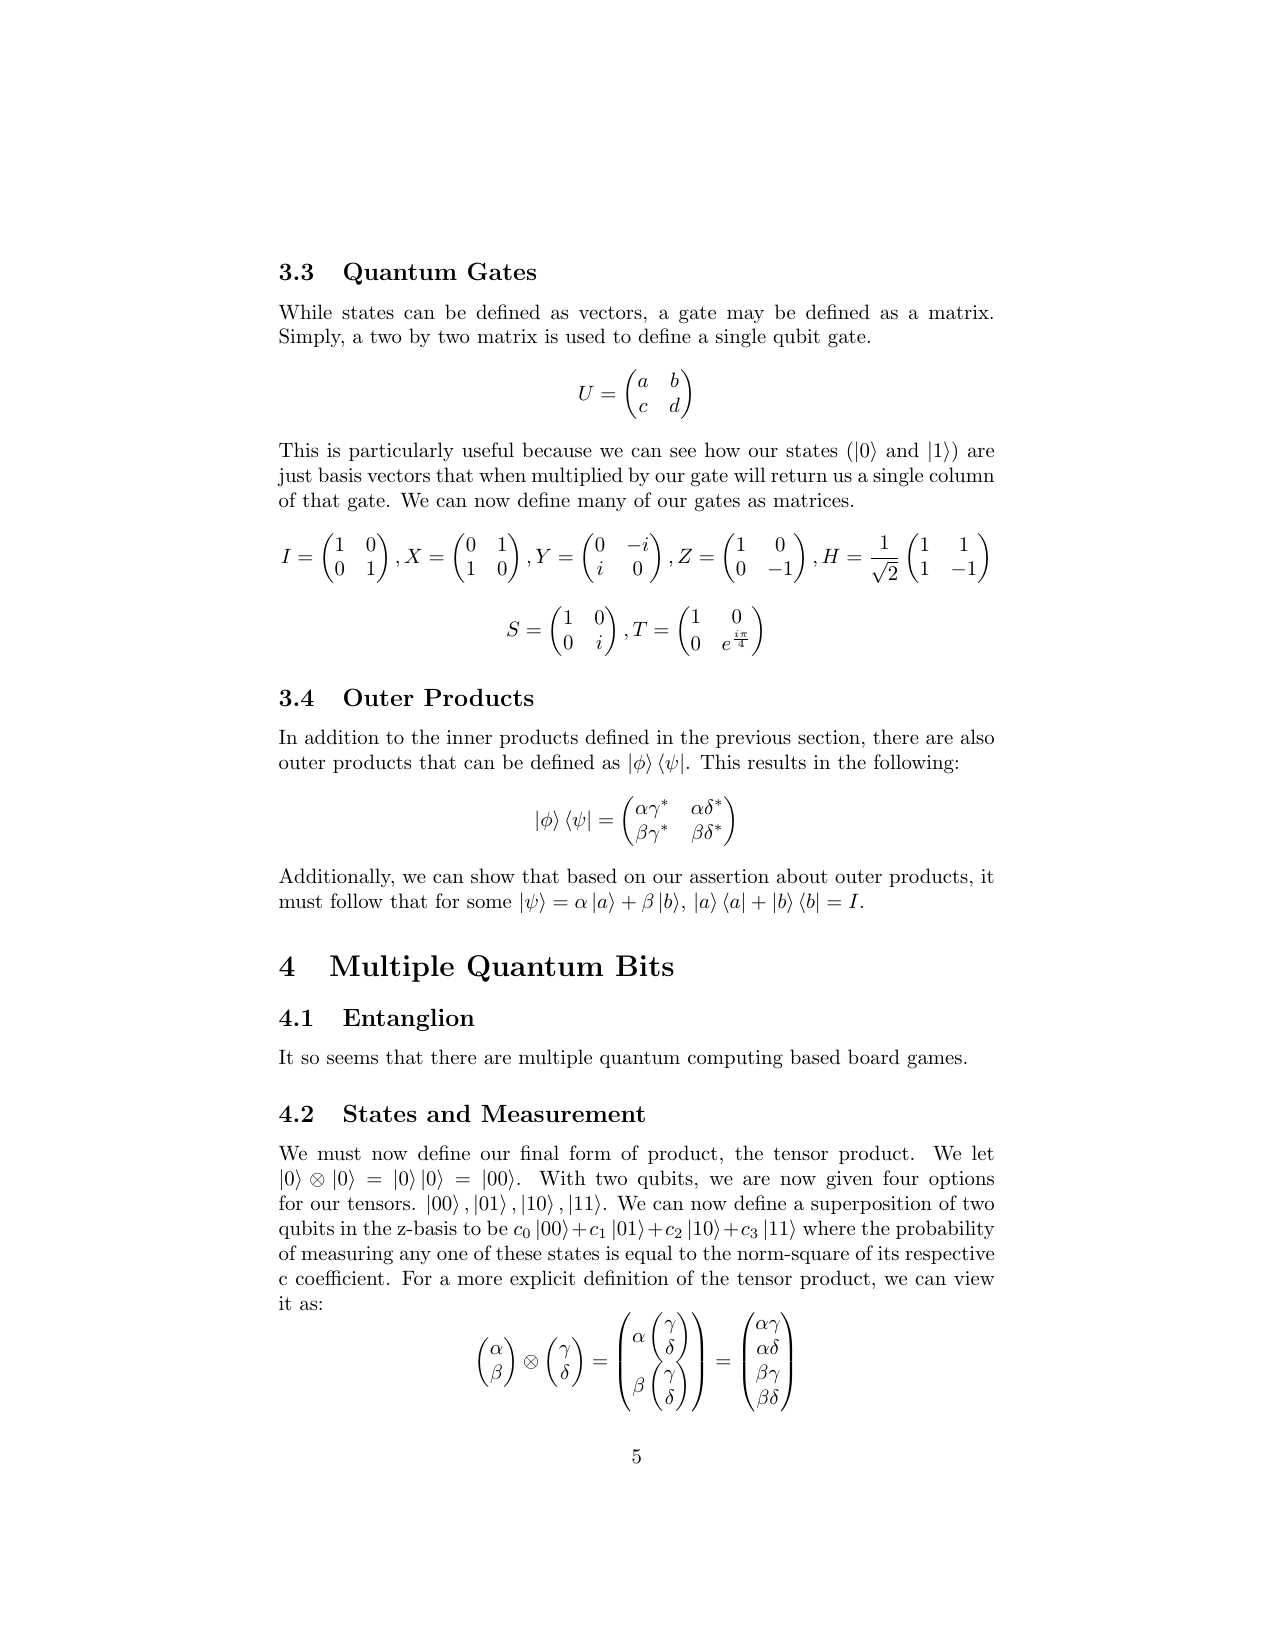
\includegraphics[width=\textwidth, keepaspectratio, trim=1cm 1cm 1cm 1cm, clip]{output_page-05.png}
\end{column}

\end{columns}

\end{frame}

%%%%%%%%%%%%%%%%%%%%%%%%%%%%%%%%%%%%%%%%%%%%%%%%%%%%%%%%%%%%%%%%%%
\begin{frame}
\frametitle{Conclusion}

\begin{block}{}
    \begin{itemize}
        \item Markup Languages are very powerful for rendering text in comprehensible formats. 
        \item These formats can be used for many tasks, from taking notes, to hosting websites.
        \item Tools like Pandoc can be used to transform between formats.
        \item Organizations like arXiv support multiple formats depending on user preference.
    \end{itemize}
\end{block}

\end{frame}

\end{document}
